\section{Task--Nuisance Geometry and Information Collapse}
\label{sec:geometry}

Let $e\sim\Pi$ index an observed group or latent subpopulation. The audit fixes the task contrast, admissible nuisance variations, and common task-coordinate normalization. Information describes the task distinction remaining after nuisance adjustment.

\subsection{Task Information After Nuisance Profiling}
\label{sec:task-information}

Consider a local model $P_{\theta,\mu,e}$ with task parameter $\theta$ and nuisance parameter $\mu$. A likelihood score measures the local change in log likelihood as a parameter varies. At $P_e=P_{0,0,e}$, assume differentiability in quadratic mean, with centered, square-integrable task-score vector $s_{T,e}$ and nuisance-score vector $s_{N,e}$. Let $\mathcal T_{N,e}$ be the closed span of admissible nuisance scores in $L^2(P_e)$, with inner product $\langle f,g\rangle_e=\E_{P_e}[fg]$, and let $\Pi_{\mathcal T_{N,e}}$ denote orthogonal projection onto that span. The \textbf{efficient task score} and its information are
\begin{equation}
\begin{aligned}
s^{\eff}_{T,e}&=s_{T,e}-\Pi_{\mathcal T_{N,e}}s_{T,e},\\
F_e:=F^{\eff}_{T\mid N,e}
&=\E_{P_e}[s^{\eff}_{T,e}(s^{\eff}_{T,e})^\top]
=J_{TT,e}-J_{TN,e}J_{NN,e}^{-1}J_{NT,e}.
\end{aligned}
\label{eq:efficient-score-information}
\end{equation}
The projection acts componentwise. The Schur expression applies when finite nuisance scores span $\mathcal T_{N,e}$ and $J_{NN,e}\succ0$, with $J_{AB,e}=\E_{P_e}[s_{A,e}s_{B,e}^{\top}]$ \citep{bickel1993efficient,tsiatis2006semiparametric,cox1987parameter}. Write $\lambda_e=\lambda_{\min}(F_e)$ for the weakest task information. A zero eigenvalue identifies a task direction contained in the nuisance span.

For scalar task and nuisance scores with positive raw information, their Fisher correlation $\rho_e=J_{TN,e}/\sqrt{J_{TT,e}J_{NN,e}}$ gives
\begin{equation}
F_e=J_{TT,e}(1-\rho_e^2),
\qquad
\underbrace{F_e/J_{TT,e}}_{\text{surviving-information fraction}}=1-\rho_e^2.
\label{eq:surviving-information-fraction}
\end{equation}
Absolute information measures remaining curvature in the declared coordinates. The fraction measures the proportion retained, lies in $[0,1]$, and is invariant to nonzero scalar rescaling of either score. It compares alignment across slices with different raw information; its feature--Schur analogue supplies the prospective selection statistic. The Fisher-Glass certificate summarizes absolute information across environments.

\subsection{Task--Nuisance Alignment and Loss--Information Separation}
\label{sec:tangency-separation}

Let $b_e,r_e$ be centered, orthogonal, unit-norm scores, with nuisance span $\operatorname{span}\{b_e\}$. For $\delta_e\ge0$, define the task score $a_e=b_e+\delta_e r_e$. Then
\begin{equation}
a_e=b_e+\delta_e r_e,
\quad J_{TT,e}=1+\delta_e^2,
\quad F_e=\delta_e^2,
\quad \frac{F_e}{J_{TT,e}}=\frac{\delta_e^2}{1+\delta_e^2}.
\label{eq:tangency-identities}
\end{equation}
Projection removes $b_e$, leaving $\delta_e r_e$. Raw information stays at least one as efficient information vanishes quadratically; $\delta_e$ measures distance from the nuisance span. When nuisance features support low observed risk, low loss coexists with arbitrarily weak efficient information, even in accurately classified populations. Appendix~\ref{app:theory-projection} gives the construction and proof. Figure~\ref{fig:geometry-tails} illustrates the population consequence: frequent near-alignment of task scores with nuisance spans produces a heavy inverse-information tail.

\begin{figure}[t]
\centering
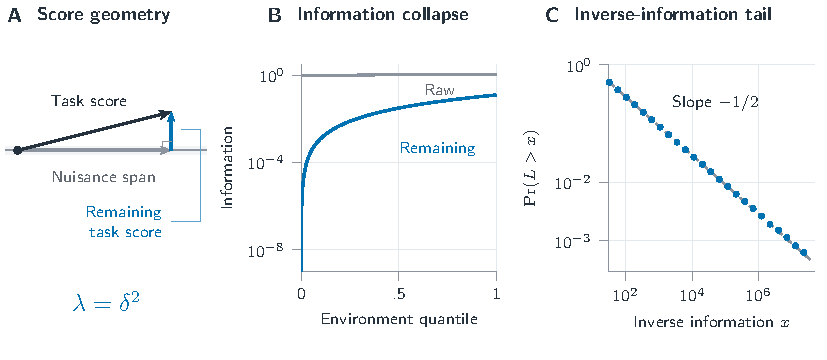
\includegraphics[width=\linewidth]{figures/fig02_geometry_tails.pdf}
\caption[Synthetic illustration of the geometric tail law]{\textbf{Near-alignment produces a heavy inverse-information tail.}
(A) Projection leaves a residual score of norm $\delta$, giving information $\lambda=\delta^2$. (B) Raw information $1+\delta^2$ remains near one as $\lambda$ approaches zero. (C) Empirical survival probabilities (blue) follow the $x^{-1/2}$ reference (dashed). Panels B--C use 300,000 environments with $\delta\sim\mathrm{Uniform}(0,0.35)$ and $L=(\delta^2+10^{-12})^{-1}$.
}
\label{fig:geometry-tails}
\end{figure}
